\documentclass[aspectratio=169]{beamer}

\usetheme{Boadilla}
\usecolortheme{dolphin}
\setbeamertemplate{navigation symbols}{}
\setbeamertemplate{footline}[frame number]

\usepackage{amsmath,amssymb}
\usepackage{graphicx}

\graphicspath{
  {../../output/model/}
  {../../output/graphs/}
  {../../output/graphs/model/}
  {../../output/graphs/descriptives/}
  {output/model/}
  {output/graphs/}
  {output/graphs/model/}
  {output/graphs/descriptives/}
}

\title[AI \& Labor Market Risk]{Present Day, Present Time:\\
  AI Exposure \& Labor Market Risk}

\date{}

\definecolor{myred}{RGB}{215,48,39}
\definecolor{mygreen}{RGB}{26,150,65}
\definecolor{mygray}{RGB}{120,120,120}

\begin{document}

% =============================================================================
%  TITLE
% =============================================================================
\begin{frame}
  \maketitle
  \vspace{-3cm}
  \centering
  
\includegraphics[width=0.4\linewidth]{starting_page.png}
\end{frame}

% =============================================================================
%  ICEBREAKER
% =============================================================================
\begin{frame}{What's Going On}

\textbf{November 2022: ChatGPT launches.}

\bigskip
Millions of people start using AI to do things that \emph{people get paid to do}.

\bigskip
\textbf{Some workers are much more exposed than others.}

\bigskip
\large\textbf{Did it cost them?}

\bigskip\hrule\medskip
\normalsize
Where I got the idea: the \textbf{offshoring} literature from trade economics.
\begin{itemize}
  \item Grossman \& Rossi-Hansberg (2008): offshoring works at the \emph{task} level
  \item Ottaviano, Peri \& Wright (2013): different workers, different cutoffs
\end{itemize}

\medskip
AI is the same story, new technology ---
\textbf{``offshoring'' your tasks to Claudeland, GPTopia, Geminia\ldots}

\end{frame}

% =============================================================================
%  TOY MODEL (condensed)
% =============================================================================
\begin{frame}{}
\centering
\vspace{0.8cm}
{\Huge\bfseries Toy Model Time!}\\[1.2cm]

\includegraphics[height=0.55\textheight]{toy_model.png}
\end{frame}

% --- Model in one slide ---
\begin{frame}{A Task-Based Model (Setup)}

\begin{itemize}
  \item Tasks $i\in[0,1]$ ordered by AI susceptibility;
        workers of type $i^*$ specialize in task $i^*$

  \medskip
  \item CES production:
  $\;Y = \bigl[\int_0^1 y(i)^{(\sigma-1)/\sigma}\,di\bigr]^{\sigma/(\sigma-1)}$

  \medskip
  \item Human supply of task $i$: $f(i)$ (fixed).
        Pre-AI wage:
  \[
    w_0(i^*) = P_Y\!\left(\frac{Y_0}{f(i^*)}\right)^{\!1/\sigma}
    \qquad\text{(scarce tasks $\rightarrow$ higher wage)}
  \]

  \medskip
  \item \textbf{AI enters as a supply shock:} adds $s(i)\geq 0$ to tasks
        below the capability frontier $I^*$
  \[
    s'(i)<0 \;\text{ for }i<I^*,
    \qquad s(i)=0 \;\text{ for }i\geq I^*
  \]
\end{itemize}

\end{frame}

% --- Post-AI ---
\begin{frame}{Post-AI Wages}

Effective supply $\bar y(i) = f(i)+s(i)$, \quad output expands to $\bar Y > Y_0$.

\[
  \boxed{w_1(i^*) = P_Y\!\left(\frac{\bar Y}{f(i^*)+s(i^*)}\right)^{\!1/\sigma}}
\]

\medskip
\begin{columns}[t]
\column{0.32\textwidth}
  \textbf{\textcolor{mygreen}{Above $I^*$}}\\[3pt]
  $s=0$ $\rightarrow$ only $\bar Y\uparrow$\\
  Wages \textcolor{mygreen}{rise}

\column{0.34\textwidth}
  \textbf{\textcolor{myred}{Deep inside $[0,I^*)$}}\\[3pt]
  $s/f$ large $\rightarrow$ denom.\ outpaces numer.\\
  Wages \textcolor{myred}{fall}

\column{0.32\textwidth}
  \textbf{\textcolor{mygreen}{Near $I^*$ from below}}\\[3pt]
  $s\approx 0$ $\rightarrow$ output growth dominates\\
  Wages still \textcolor{mygreen}{rise}
\end{columns}
\end{frame}

\begin{frame}{Graphically}
    \centering

\includegraphics[width=1.0\linewidth]{fig_postai.png}
\end{frame}
% =============================================================================
%  BRIDGE
% =============================================================================
\begin{frame}{}
  \Large
  \centering
  The model says high-exposure workers should see worse outcomes post-2022.

  \bigskip
  \large
  \textcolor{red}{\textbf{Let's test it.}}
\end{frame}

% =============================================================================
%  DATA
% =============================================================================
\begin{frame}{Data}

\begin{columns}[t]
\column{0.50\textwidth}
  \textbf{CPS-ASEC} (via IPUMS)
  \begin{itemize}
    \item 500K+ person-year obs, 2018--2025
    \item Ages 22--65, labor force participants
    \item Outcomes:
    \begin{itemize}
      \item Unemployment
      \item Log real annual wages (CPI-U deflated)
    \end{itemize}
  \end{itemize}

\column{0.48\textwidth}
  \textbf{AI Exposure} (Eloundou et al.\ 2024)
  \begin{itemize}
    \item Occupation-level LLM exposure score ($\beta_o$)
    \item GPT-4 annotated, O*NET task database
    \item 0 (eg. construction workers) to 0.80~ (eg. programmers)
    \item Time-invariant, assigned at occ.\ level
  \end{itemize}
\end{columns}

\end{frame}

% --- Who's exposed? ---
\begin{frame}{Who's Exposed?}

\begin{columns}[c]
\column{0.55\textwidth}
  \centering
  
\includegraphics[width=\linewidth]{kdensity_beta_overall.pdf}
\column{0.42\textwidth}
  \small
  \begin{itemize}
    \item Most workers cluster at low--moderate exposure
    \item A long right tail: programmers, legal, financial analysts
    \medskip
    \item Each observation = one worker-year\\
          (density reflects the \emph{worker} distribution)
  \end{itemize}
\end{columns}

\end{frame}

% --- College vs Non-college exposure ---
\begin{frame}{Exposure by Education}

\begin{columns}[c]
\column{0.55\textwidth}
  \centering
  
\includegraphics[width=\linewidth]{kdensity_beta_education.pdf}
\column{0.42\textwidth}
  \small
  \begin{itemize}
    \item College workers shifted right ---
          more exposed on average
    \medskip
    \item But substantial overlap ---
          both groups contain high- and low-exposure workers
    \medskip
    \item This matters: the asymmetric wage result
          (non-college hit, college not) is \emph{not} simply
          because the groups face different exposure
  \end{itemize}
\end{columns}

\end{frame}

% --- Raw time series ---
\begin{frame}{Eyeball Test: Unemployment by Exposure Quartile}

\centering

\includegraphics[width=0.78\linewidth]{unemp_by_quartile_post2022.pdf}

\smallskip
{\small Raw means, no regression.  Q4 (highest exposure) diverges from Q1 after 2022 ---
the pattern the model predicts.}

\end{frame}

% =============================================================================
%  EMPIRICAL STRATEGY
% =============================================================================
\begin{frame}{Empirical Strategy}

\begin{columns}[c]
\column{0.54\textwidth}
  \[
    Y_{it} = \alpha + \!\!\sum_{t \neq 2022}\!\! \beta_t
    \bigl(\mathbf{1}[t] \times \mathrm{AIExp}_i\bigr)
    + X_{it}'\Gamma + \varepsilon_{it}
  \]
  {\small\color{blue}
    $X_{it}$: sex, education, state$\times$year FEs\\
    SEs clustered by occupation \quad Baseline: 2022 $(\beta_{2022}\equiv 0)$\\[6pt]
    Four control specs: (1) none $\rightarrow$ (2) sex $\rightarrow$
    (3) sex+educ $\rightarrow$ \textbf{(4) + state$\times$year}
  }

\column{0.43\textwidth}
  \small
  \begin{itemize}
    \item Year-by-year interaction with AI exposure
          $\rightarrow$ event-study coefficients $\hat\beta_t$
    \medskip
    \item Pre-2022 $\hat\beta_t$: tests for parallel trends
    \item Post-2022 $\hat\beta_t$: possible effects from AI
    \medskip
    \item \textbf{Education heterogeneity:}
          estimate separately for college vs.\ non-college
  \end{itemize}
\end{columns}

\end{frame}

% =============================================================================
%  RESULTS
% =============================================================================

% --- Unemployment ---
\begin{frame}{Result 1: Unemployment}

\begin{columns}[c]
\column{0.60\textwidth}
  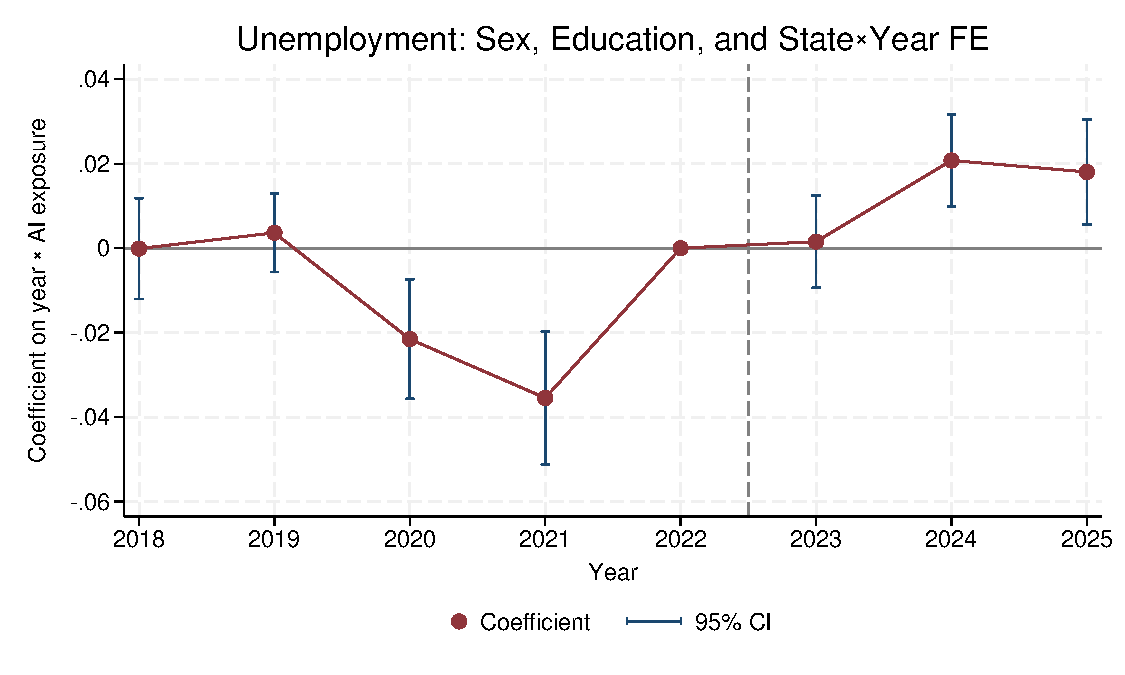
\includegraphics[width=\linewidth]{unemployment_stateYFE_plot.pdf}
\column{0.37\textwidth}
  \small
  \begin{itemize}
    \item Pre-2022: flat (2018--19)
    \item 2020--21: \textcolor{mygreen}{negative} ---
          AI-exposed jobs are remote-compatible, shielded from COVID layoffs
    \medskip
    \item \textbf{Post-2022: reversal}
    \begin{itemize}
      \item 2024: $+0.021^{***}$
      \item 2025: $+0.018^{***}$
    \end{itemize}
    \item $\approx$ 6\% increase relative to 3.4\% baseline
    \item Robust across all four specs
  \end{itemize}
\end{columns}

\end{frame}

% --- Wages ---
\begin{frame}{Result 2: Wages}

\begin{columns}[c]
\column{0.60\textwidth}
  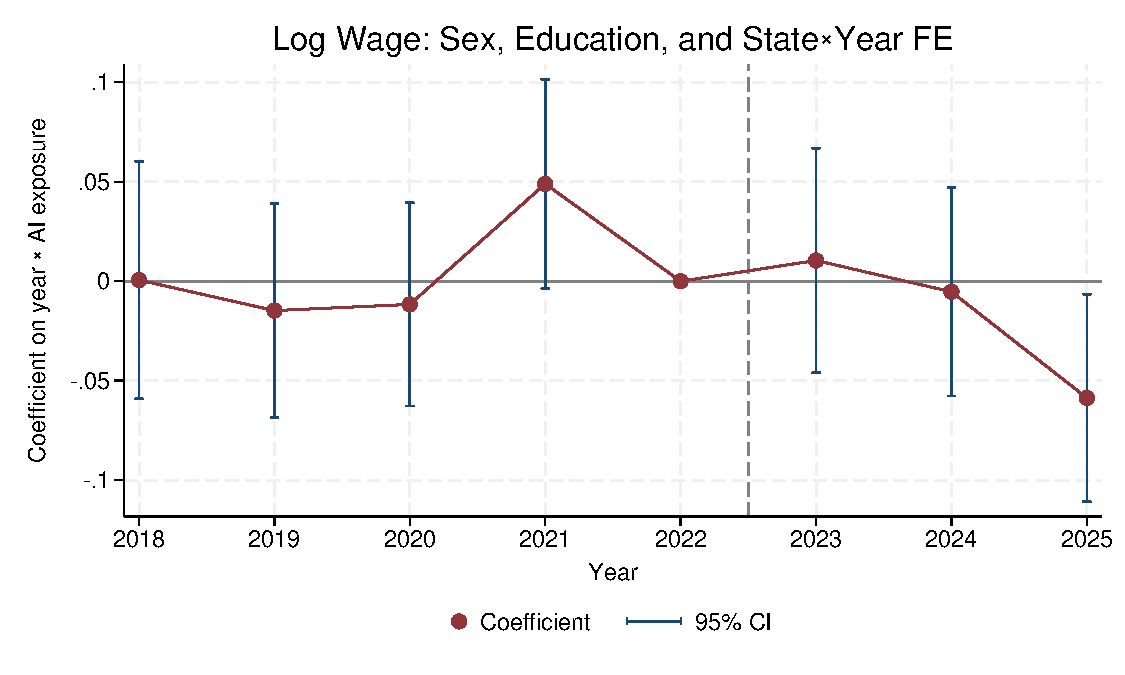
\includegraphics[width=\linewidth]{logwage_stateYFE_plot.pdf}
\column{0.37\textwidth}
  \small
  \begin{itemize}
    \item Pre-2022: flat --- clean parallel trends
    \medskip
    \item Post-2022: compression emerges late
    \begin{itemize}
      \item 2025: $-0.059^{**}$ (preferred spec only)
    \end{itemize}
    \item Weaker and later than unemployment
    \item Not significant under looser specs
    \medskip
    \item Wage adjustment lags behind employment adjustment
  \end{itemize}
\end{columns}

\end{frame}

% --- Education Het: Unemployment ---
\begin{frame}{Who Bears the Burden? Unemployment by Education}

\begin{columns}[c]
\column{0.60\textwidth}
  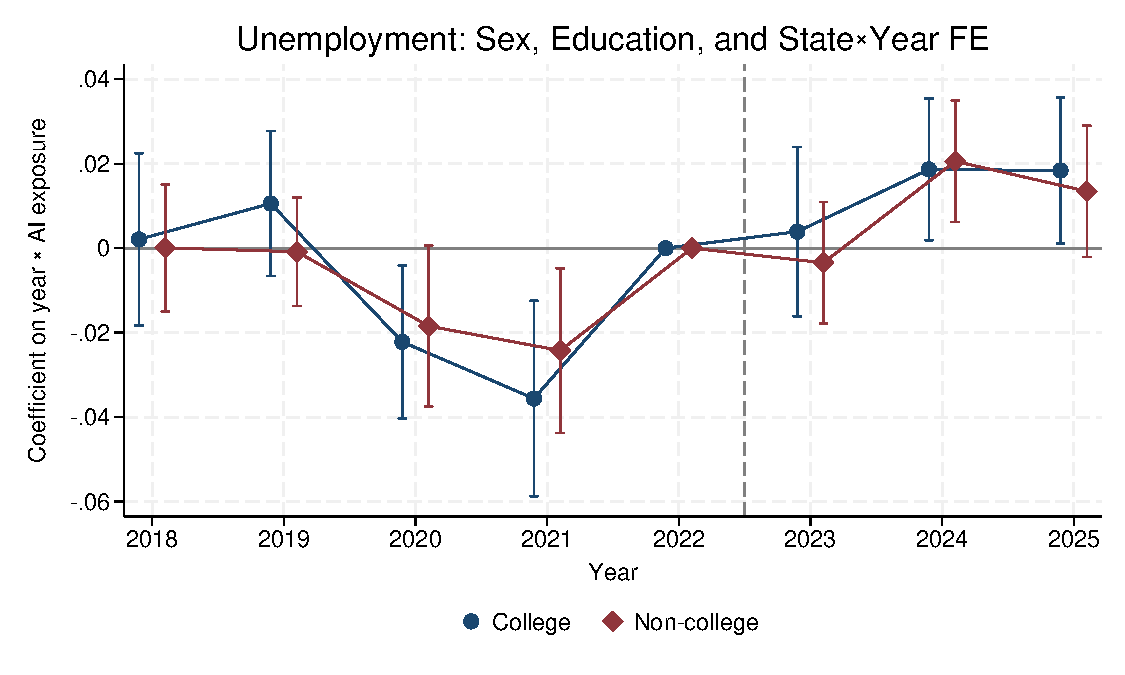
\includegraphics[width=\linewidth]{unemp_stateYFE_plot_colComb.pdf}
\column{0.37\textwidth}
  \small
  \begin{itemize}
    \item \textbf{Symmetric}: both groups see comparable
          post-2022 unemployment increases
    \medskip
    \item College: $+0.018^{**}$ (2024, 2025)
    \item Non-college: $+0.020^{***}$ (2024), $+0.014^{*}$ (2025)
    \medskip
    \item CIs overlap --- no significant difference
    \item AI unemployment risk is \textbf{broadly shared}
  \end{itemize}
\end{columns}

\end{frame}

% --- Education Het: Wages ---
\begin{frame}{Who Bears the Burden? Wages by Education}

\begin{columns}[c]
\column{0.60\textwidth}
  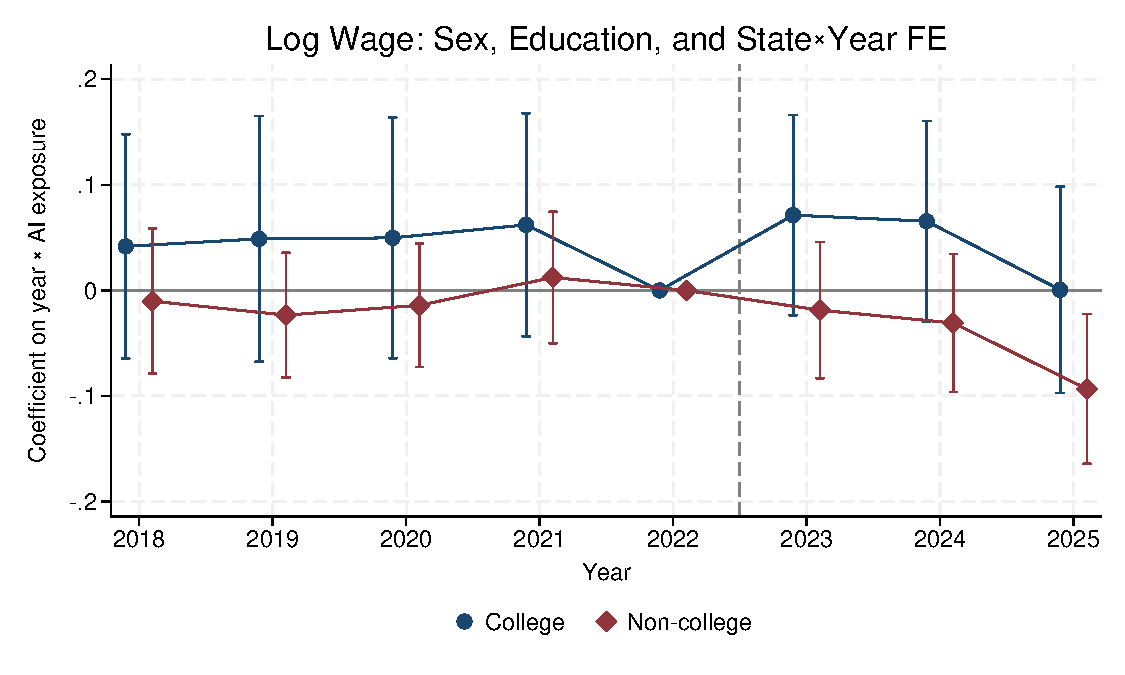
\includegraphics[width=\linewidth]{lw_stateYFE_plot_colComb.pdf}
\column{0.37\textwidth}
  \small
  \begin{itemize}
    \item \textbf{Asymmetric}:
    \medskip
    \item College: post-2022 coefficients positive,
          insignificant --- no compression
    \medskip
    \item \textbf{Non-college 2025:}
          $-0.094^{***}$ (preferred spec)
    \item Grows more significant with richer FEs
    \medskip
    \item Unemployment shared; wage compression
          concentrated among non-college workers
  \end{itemize}
\end{columns}

\end{frame}

% =============================================================================
% THANK YOU
% =============================================================================
\begin{frame}{}
\centering
\vspace{1.2cm}
{\Large Thank you!}\\[0.8cm]
{\normalsize Questions welcome.}\\[1.2cm]

\begin{columns}[c]
\column{0.48\textwidth}
  \centering
  {\small\color{mygray}\itshape Bottom line:}\\[4pt]
  {\normalsize AI works like offshoring ---\\
  task-level supply shock,\\
  heterogeneous exposure}

\column{0.48\textwidth}
  \centering
  {\small\color{mygray}\itshape What the data shows:}\\[4pt]
  {\normalsize Unemployment: broad, robust, both groups\\
  Wages: late, concentrated on non-college}
\end{columns}
\end{frame}

% =============================================================================
% BACKUP — THE DIRTY WORK
% =============================================================================
\appendix

\begin{frame}{}
\centering
\vspace{2cm}
{\large\color{mygray}\itshape Backup: The Dirty Work}\\[0.5cm]
{\small\color{mygray} Full derivation, three-group analysis, $I^*$ discussion}
\end{frame}

% --- B1: Full Pre-AI Derivation ---
\begin{frame}{Derivation: Pre-AI Equilibrium}

\textbf{Step 1.} Cost minimization $\rightarrow$ FOC:
$\;p_0(i)=\mu\cdot(Y/y(i))^{1/\sigma}$, \quad $\mu=P_Y$ in competitive eq.

\medskip
\textbf{Step 2.} Task demand: $\;y^d(i)=Y(P_Y/p_0(i))^{\sigma}$

\medskip
\textbf{Step 3.} Market clearing $y^d(i)=f(i)$:
\[
  p_0(i) = P_Y\!\left(\frac{Y}{f(i)}\right)^{\!1/\sigma}
\]

\textbf{Step 4.} Plug $y(i)=f(i)$ into CES $\rightarrow$ output is pinned:
\[
  \boxed{Y_0 = \left[\int_0^1 f(i)^{(\sigma-1)/\sigma}\,di
  \right]^{\!\sigma/(\sigma-1)}}
\]

$Y_0$ depends only on worker distribution $f$ --- not on prices.

\end{frame}

% --- B2: Post-AI Derivation ---
\begin{frame}{Derivation: Post-AI Equilibrium}

\textbf{Step 5.} AI adds supply $s(i)$. Effective supply:
$\bar y(i)=f(i)+s(i)$.

\medskip
Repeat Steps 1--4 with $\bar y$ in place of $f$:
\[
  \bar Y = \left[\int_0^1 (f(i)+s(i))^{(\sigma-1)/\sigma}\,di
  \right]^{\!\sigma/(\sigma-1)} > Y_0
\]

Post-AI wage:
\[
  \boxed{w_1(i^*) = P_Y\!\left(\frac{\bar Y}{f(i^*)+s(i^*)}\right)^{\!1/\sigma}}
\]

\medskip
Wage ratio:
\[
  \frac{w_1(i^*)}{w_0(i^*)}
  = \underbrace{\left(\frac{\bar Y}{Y_0}\right)^{\!1/\sigma}}_{\text{output expansion}>1}
  \cdot
  \underbrace{\left(\frac{f(i^*)}{f(i^*)+s(i^*)}\right)^{\!1/\sigma}}_{\text{supply effect}\leq 1}
\]

\end{frame}

% --- B3: Three-Group Formal ---
\begin{frame}{Three-Group Analysis (Formal)}

\small
\textbf{Group 1} ($i^*\geq I^*$, $s=0$): \quad
$w_1/w_0 = (\bar Y/Y_0)^{1/\sigma} > 1$ --- uniform gain.

\bigskip
\textbf{Group 2} ($i^*<I^*$, $s/f$ large): \quad
Compression whenever $\;s(i^*)/f(i^*) > \bar Y/Y_0 - 1$.

Because $\bar Y/Y_0$ is a CES average over \emph{all} tasks (most with $s\!=\!0$),
while $s/f$ is concentrated on AI-supplied tasks, this condition holds for
heavily exposed workers.

\bigskip
\textbf{Group 3} ($i^*<I^*$, $s/f$ small): \quad
Near $I^*$, $s\to 0$ so supply effect $\approx 1$ and output expansion
dominates $\rightarrow$ \textcolor{mygreen}{gain} despite $i^*<I^*$.

\bigskip
\textbf{Threshold $\hat\imath < I^*$:}\quad
$s(\hat\imath)/f(\hat\imath) = \bar Y/Y_0 - 1$.\\
Winners: $i^*>\hat\imath$.  Losers: $i^*<\hat\imath$.
The boundary lies \emph{strictly below} $I^*$.

\end{frame}

% --- B4: I* Discussion ---
\begin{frame}{Further Discussion of $I^*$}

\begin{columns}[t]
\column{0.50\textwidth}

  \textbf{As AI improves, $I^*$ shifts right}\\[4pt]
  More workers exposed, deeper compression,
  $\hat\imath$ shifts rightward.

  \medskip
  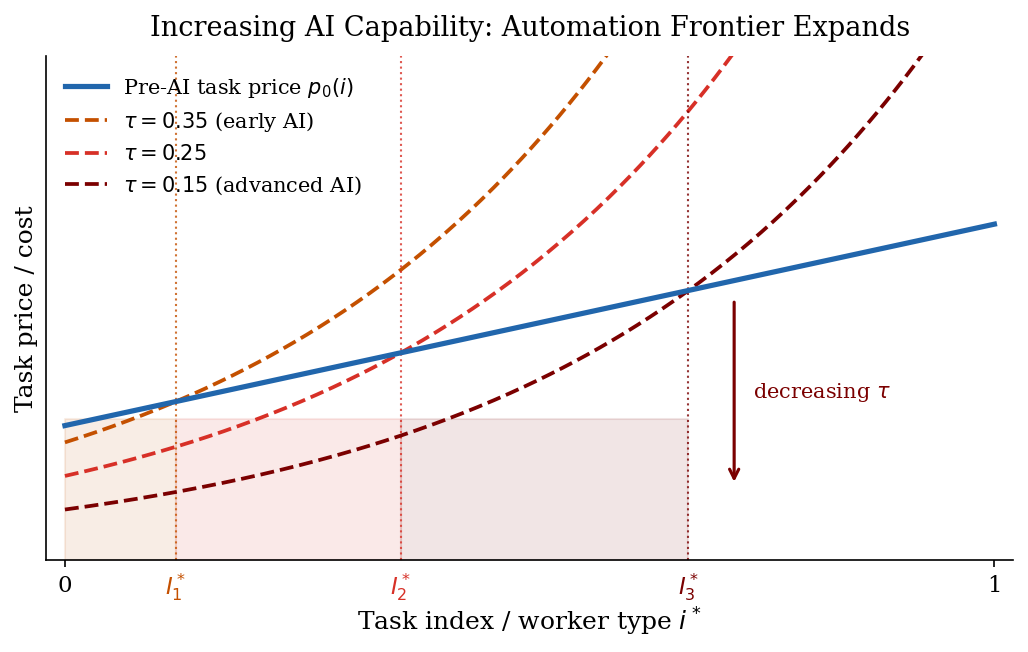
\includegraphics[width=\linewidth]{fig_capability.png}
  {\tiny Each curve: $w_1$ for a different $I^*$. Higher $I^*\rightarrow$ wider compression.}

\column{0.48\textwidth}

  \textbf{Non-monotone $f(i)$: scattered effects}\\[4pt]
  If many workers cluster in a mid-complexity task, the local $s/f$ ratio
  drops, creating pockets where workers gain even inside $[0,I^*)$.

  \medskip
  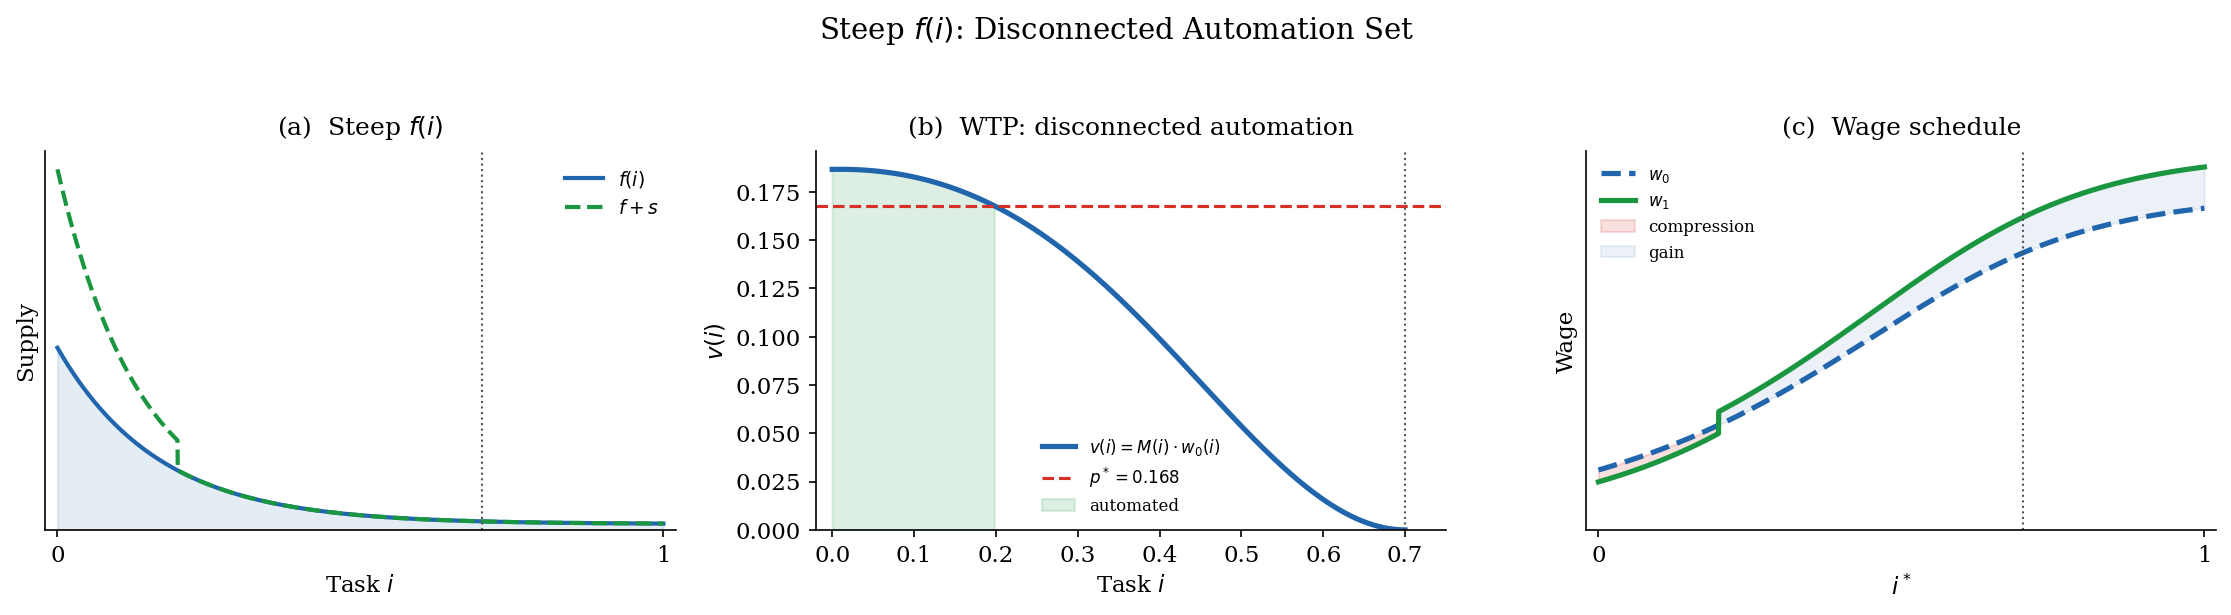
\includegraphics[width=\linewidth]{fig_multiple.png}
  {\tiny Bump in $f$ near $i\!\approx\!0.55$: gain pocket inside the frontier.}

\end{columns}

\end{frame}

\end{document}
